\documentclass[5pt]{article}
\usepackage{multicol,multirow}
\usepackage{graphicx} % Required for inserting images
\usepackage[margin=0.75cm]{geometry}
\usepackage{xcolor}
\usepackage{amsmath}
\usepackage{mathtools}
\usepackage{relsize}

\usepackage[english]{babel}
\newtheorem{theorem}{Theorem}

\usepackage{empheq}
\usepackage{amsfonts}

\usepackage{array}
\usepackage[inline]{enumitem}

\usepackage{tkz-euclide}
\usepackage{tikz}
\usepackage{rotating}

\definecolor{LightGray}{gray}{0.9}

\usepackage{minted}
\newcolumntype{L}{>{\footnotesize}l}
\newcolumntype{C}{>{\ttfamily\footnotesize}l}

\DeclarePairedDelimiter\abs{\lvert}{\rvert}%
\DeclarePairedDelimiter\norm{\lVert}{\rVert}%

\makeatletter
\let\oldabs\abs
\def\abs{\@ifstar{\oldabs}{\oldabs*}}

\newcommand{\tr}[3]{
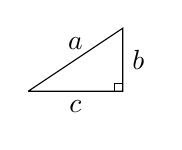
\begin{tikzpicture}[scale=0.40]
    \coordinate [] (A) at (-1.5cm,-1.cm);
    \coordinate [] (C) at (1.5cm,-1.0cm);
    \coordinate [] (B) at (1.5cm,1.0cm);
    \draw (A) -- node[above] {$a$} (B) -- node[right] {$b$} (C) -- node[below] {$c$} (A);
    \draw (1.25cm,-1.0cm) rectangle (1.5cm,-0.75cm);
\end{tikzpicture}
}


\begin{document}


\begin{center}
     \Large{\textbf{Machine Learning in Python}}\\
     \small{Last Update: \today}\hfill\small{ Maximilien Notz}
     \noindent\rule{20.2cm}{0.4pt}
\end{center}


\begin{multicols}{2}
\setcounter{secnumdepth}{0}

\subsection{Numpy}
\subsection{Pytorch}
\subsubsection{Tensor}
Let \texttt{t} be a pytorch tensor and the following are from \texttt{torch}:\\
\begin{tabular}{C L}
.randn(s)     & Create a random tensor of rank 1\\
.ones(s)      & Create a tensor of ones of rank 1\\
.zeros(s)     & Create a tensor of zeros of rank 1\\
.cat(lst,dim=d) & Concatenate the tensors in lst along dimension \texttt{d}\\
.mul(t1,t2)     & Element-wise multiplication of \texttt{t1} and \texttt{t2}\\
.add(t1,t2)     & Element-wise addition of \texttt{t1}\\
t.size()     & Return the size of the tensor \texttt{t}\\
t.view(s)     & Reshape the tensor \texttt{t} to the shape
\end{tabular}

\subsubsection{Deep Learning}
All the following are in \texttt{torch.nn}:\\
\begin{tabular}{C L}
.linear(m, n)     & Apply a afine linear transformation object with \texttt{m}\\
                  & inputs and \texttt{n} outputs.\\
.conv1d(m, n, k)  & Apply 1D convolution with \texttt{m} input chanels and \texttt{n}\\
                  & output chanels with a kernel \texttt{k}.\\
.conv2d(m, n, k)  & Apply 2D convolution with \texttt{m} input chanels and \texttt{n}\\
                  & output chanels with a kernel \texttt{k}.\\
.conv3d(m, n, k)  & Apply 3D convolution with \texttt{m} input chanels and \texttt{n}\\
                  & output chanels with a kernel \texttt{k}.\\
\end{tabular}
\texttt{print(obj,sep='|',end='.',file=sys.stdout,flush=False)}
Prints \texttt{obj} to the specified \texttt{file} with a separator \texttt{sep} between objects and an ending character \texttt{end} at the end

\subsubsection{Activation Function}
All \texttt{Pytorch} are not performed in place unless we add the argument \texttt{inplace=False}.\\
\begin{tabular}{C L}
.Sigmoid()                      & $\sigma(x)=\frac{1}{1+e^{-x}}$\\
.ReLU()                         & $\text{ReLU}(x)=\max(0,x)$\\
.LeakyReLU(negative\_slope=m)   & $\text{LeakyReLU}(x)=\begin{cases}x & x>0\\ mx & x\leq0 \end{cases}$\\
.Tanh()                         & $\tanh(x)=\frac{e^x-e^{-x}}{e^x+e^{-x}}$
\end{tabular}

\subsubsection{Regularization}
\begin{tabular}{C L}
.Dropout(p=P)   & Dropout regularization with probability \texttt{P}\\
.BatchNorm()    & Batch normalization\\
\end{tabular}

\subsection{Scikit Learn}
\subsubsection{K-Fold Cross-Validation}
Snippet for K-Fold Cross-Validation using Scikit Learn:
\begin{minted}[bgcolor=LightGray]{Python}
kfold = KFold(n_splits=5, shuffle=True)
scores = cross_val_score(model, X, y, cv=kfold, 
    scoring='accuracy')

print("Folds accuracy:", scores)
print("Mean Accuracy:", np.mean(scores))
\end{minted}

\subsection{Optuna}
Optuna is a powerful hyperparameter optimization framework that automates the process of searching for the best hyperparameters for machine learning models.
\subsubsection{General Shape}
\begin{minted}[bgcolor=LightGray]{Python}
def Objective(trial):
    # Define hyperparameters to optimize
    param1 = trial.suggest_float('param1', low, high)
    param2 = trial.suggest_int('param2', low, high)
        
    # Create and train your model
    model = YourModel(_param1=param1, _param2=param2)
    kfold = KFold(n_splits=5, shuffle=True)
    scores = cross_val_score(model, X, y, cv=kfold, 
            scoring='accuracy')

    # Evaluate the model on validation data
    score = model.score(X_val, y_val)
        
    return score
study = optuna.create_study(direction='maximize')
study.optimize(Objective, n_trials=100)
print("Best hyperparameters:", study.best_params)
fig = optuna.visualization.plot_slice(study, 
    params=["param1", "param2"])
show(fig)
\end{minted}

\subsubsection{Pruning}
Optuna pruning allows you to stop unpromising trials early, saving computational resources and speeding up the optimization process.
You can enable pruning by using \texttt{trial.should\_prune()} inside the training loop which method to check if the trial should be pruned.

\subsection{Base Models}
\subsubsection{XGBoost}
\subsubsection{LightGBM}
\subsubsection{ROCKET}
\subsubsection{MINIROCKET}




\end{multicols}
\end{document}
